\startchapter{Feature Prototype On Atlantis}
\label{chapter:newsol}

In this section we discuss the design of the prototype of dual-trace analysis. The tool prototype I built was based on the general communication model I described in last section.
This prototype consist of three main components: user interface for defining the communication type, algorithm of locating the communication events in the dual-trace, user interface and strategy to navigate the located events to the sender and receiver traces. We provide the background information of the design of each component as well as their detail design in each corresponding subsection.
\subsection{User Defined Communication Type}
In our design, we don't specify any predefined communication type but give the user ability to do that. By the user interface implemented, the user can defined their own communication type. This give the flexibility to the user to define what they are looking for. Each communication type consist of 4 system function calls. They are channel create/open in sender and receiver sides, sender's send message function and receiver's receive message function. By indicating the channel create/open functions in both sender and receiver sides, the tool can acquire the channel's identifiers. Later on the tool can match the send and received messages within a specific channel. The send and receive functions are used to located the event happened in the traces. The messages sent and received are reconstructed from the memory state when the send and receive functions are called and returned. The detail of the match algorithm will be discuss later.

\subsubsection{Function Calls in the Traces}
The called functions' name can be inspected  by  search of the symbolic name in the executable binary or any DLLs which used by the program at the time when it is traced. This functionality exists in the current Atlantis. By importing the DLLs and execution  executable binary, Atlantis can list all called functions for the users in the Functions view. From this list, users can chose the interested functions and generate their interested communication type. In Figure\ref{functionsview} there is  an action item "Add to Communication type" in the right click menu of the function entry. Figure \ref{dialog} shows the dialogue for entering the information for the adding function. As this figure shows, users can get the existing communication type list in the drop down menu. They can choose to add the current function to an exist communication type or they can add it to a new communication type by entering a new name. For the channel create/open function, the register holding the address of channel's name as input and the register holding the handle identification of the channel as output are required. For the send/receive function, the register holding the address of the send/receiver buffer, the register holding the length of the sending/receiving message and the register holding the channel's identification are required. As there are 4 functions for each communication type users have to repeat this add function to communication type action for 4 times to generate one communication type.

\begin{figure}[h]
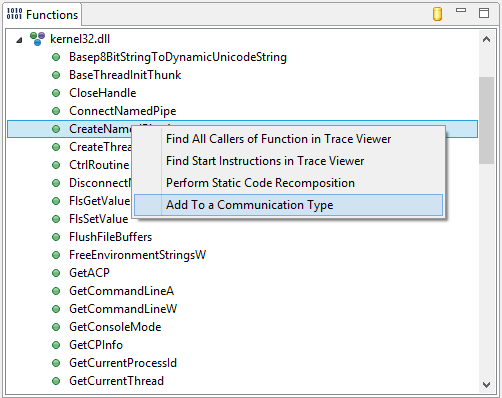
\includegraphics{Figures/functionsview}
 \caption{Add function to a Communication type from Functions View}
\label{functionsview}
\end{figure}

\begin{figure}[h]
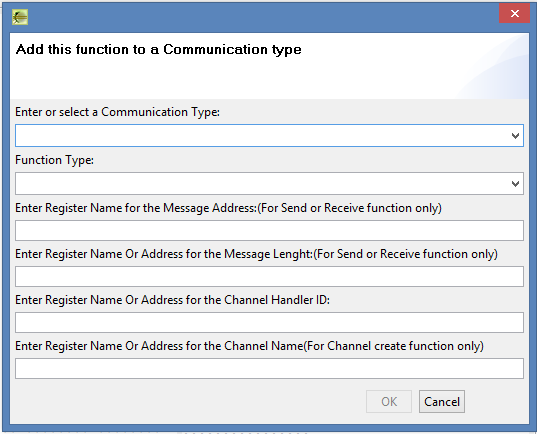
\includegraphics{Figures/dialog}
 \caption{Dialog to input information for a function adding to a communication type}
\label{dialog}
\end{figure}

\subsubsection{Communication Type Data Structure}
The defined communication type will be stored in a xml file. The list below shows the data structure of one communication type. 
\begin{lstlisting}
<messageTypesData>
    <parentFolder>.tmp</parentFolder>
    <messageTypes>
        <messageType>
            <name>namedPipe_clientsend</name>
            <sendFunction>
                <associatedFileName>Client</associatedFileName>
                <name>WriteFile</name>
                <messageAddress>RDX</messageAddress>
                <messageLengthAddress>R8</messageLengthAddress>
                <channelIdReg>RCX</channelIdReg>
            </sendFunction>
            <receiveFunction>
                <associatedFileName>Server</associatedFileName>
                <name>ReadFile</name>
                <messageAddress>RDX</messageAddress>
                <messageLengthAddress>R8</messageLengthAddress>
                <channelIdReg>RCX</channelIdReg>
            </receiveFunction>
            <sendChannelCreateFunction>
                <associatedFileName>Client</associatedFileName>
                <name>CreateFileA</name>
                <channelIdReg>RAX</channelIdReg>
                <channelNameAddress>RCX</channelNameAddress>
            </sendChannelCreateFunction>
            <receiveChannelCreateFunction>
                <associatedFileName>Server</associatedFileName>
                <name>CreateNamedPipeA</name>
                <channelIdReg>RAX</channelIdReg>
                <channelNameAddress>RCX</channelNameAddress>
            </receiveChannelCreateFunction>
        </messageType>
    </messageTypes>
</messageTypesData>
\end{lstlisting}


\subsubsection{Communication Type View}
A new view named Communication Types view is for the user defined communication types. All user defined communication type are stored in the .xml file and listed in communication type view when it's opened as shown in Figure \ref{CommunicationTypeview}. User can change the name of a communication type, remove an existing communication type or searching of the match message occurrences of selected communication type by selecting action item in the right click menu of an communication type entry. The matched messages are listed in the result window of the view. By clicking the entry of the search  result, user can navigate to it's sender or receiver's corresponding instruction line as shown in Figure\ref{searchresult}. Message content in the memory view will be shown as well.


\begin{figure}[h]
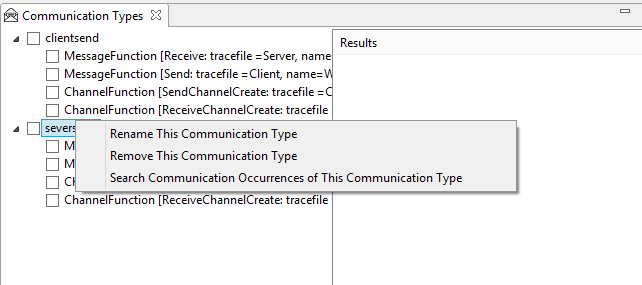
\includegraphics[scale=.9]{Figures/CommunicationTypeview}
 \caption{New View: Communication Type View}
\label{CommunicationTypeview}
\end{figure}

\begin{figure}[h]
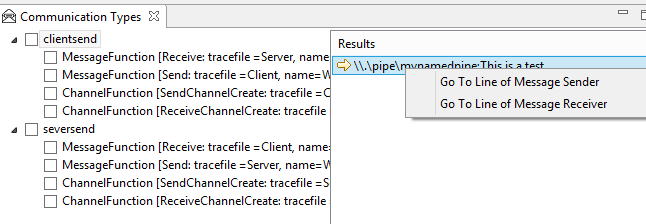
\includegraphics[scale=.9]{Figures/searchresult}
 \caption{Right Click menu to navigate to send and receive event in the traces}
\label{searchresult}
\end{figure}

\subsection{Communication Event Searching}
The communication event consists of the send message event in the sender side and receive message event in the receiver side. The communication event searching algorithm can be divided into three main steps: 1. search all channel create/open event in the sender and receiver side, save the handle id and corresponding channel name. 2. Search all message send and receive event in sender and receiver sides. 3. Matching the send/receive messages pair based on the channel names and message contents.
\subsubsection{Record opened Channel}
In this step the algorithm is supposed to search all the open channel both in the sender and receiver side. The found created channels are recorded in a map. The key of the map is the handler id of the channel and the value is the channel name. A channel in the sender and receiver sides will have different handler id but same channel name.
\subsubsection{Search send and receive Message}
All send message and receive message function calls will be found out in the trace. When a send function hit, the memory state of the hit instruction line will be reconstructed, and the message content can be get from the memory with the send message buffer address. When a receive function hit, the return line of that function is needed for getting the message content. The memory state of the function return line is reconstructed and the message content can be get  from the reconstructed memory state with the receive message buffer address.
\subsubsection{Matching the send/receive messages pair}
After the created channel and send/receive message are found out in the sender and receiver side, a matching algorithm is used to match the send/receive message pairs.
\subsubsection{Matching Event Data Structure}
The matching event is stored in cache when the tool is running. Only the most recent search result is cached currently. If users need the previous result, they need to apply the search again. The matching Event consist of two sub-events, one is message send event while the other is message receive event. Both of these two sub-events are object of BfvFileMessageMatch. BfvFileMessageMatch is an Java class extends org.eclipse.search.internal.ui.text.FileMatch. FileMatch class containing the information needed to navigate to the trace file editor. In order to show the corresponding send/receive message in the memory view, the target memory address storing the message content is set in BfvFileMessageMatch. Two more elements: message and channel name are also set in BfvFileMessageMatch which are listed in the search result. 

\subsection{Matching Event Visualization and Navigation}
The right click menu of an entry in the search result list has two action items: Go To Line of Message Sender and Go To Line of Message Receiver. Both of the action items allow users to navigate to the trace Instruction view. When the user click on these items, it will navigate to the corresponding trace sender or receiver trace instruction view.  Meanwhile the memory view jumps to the target address of the message buffer, and the memory state is reconstructed so that the message content in that buffer will be shown in the memory view.

